%\documentclass{standalone}
%\usepackage{tikz}
%\usetikzlibrary{patterns,plotmarks}
%\begin{document}
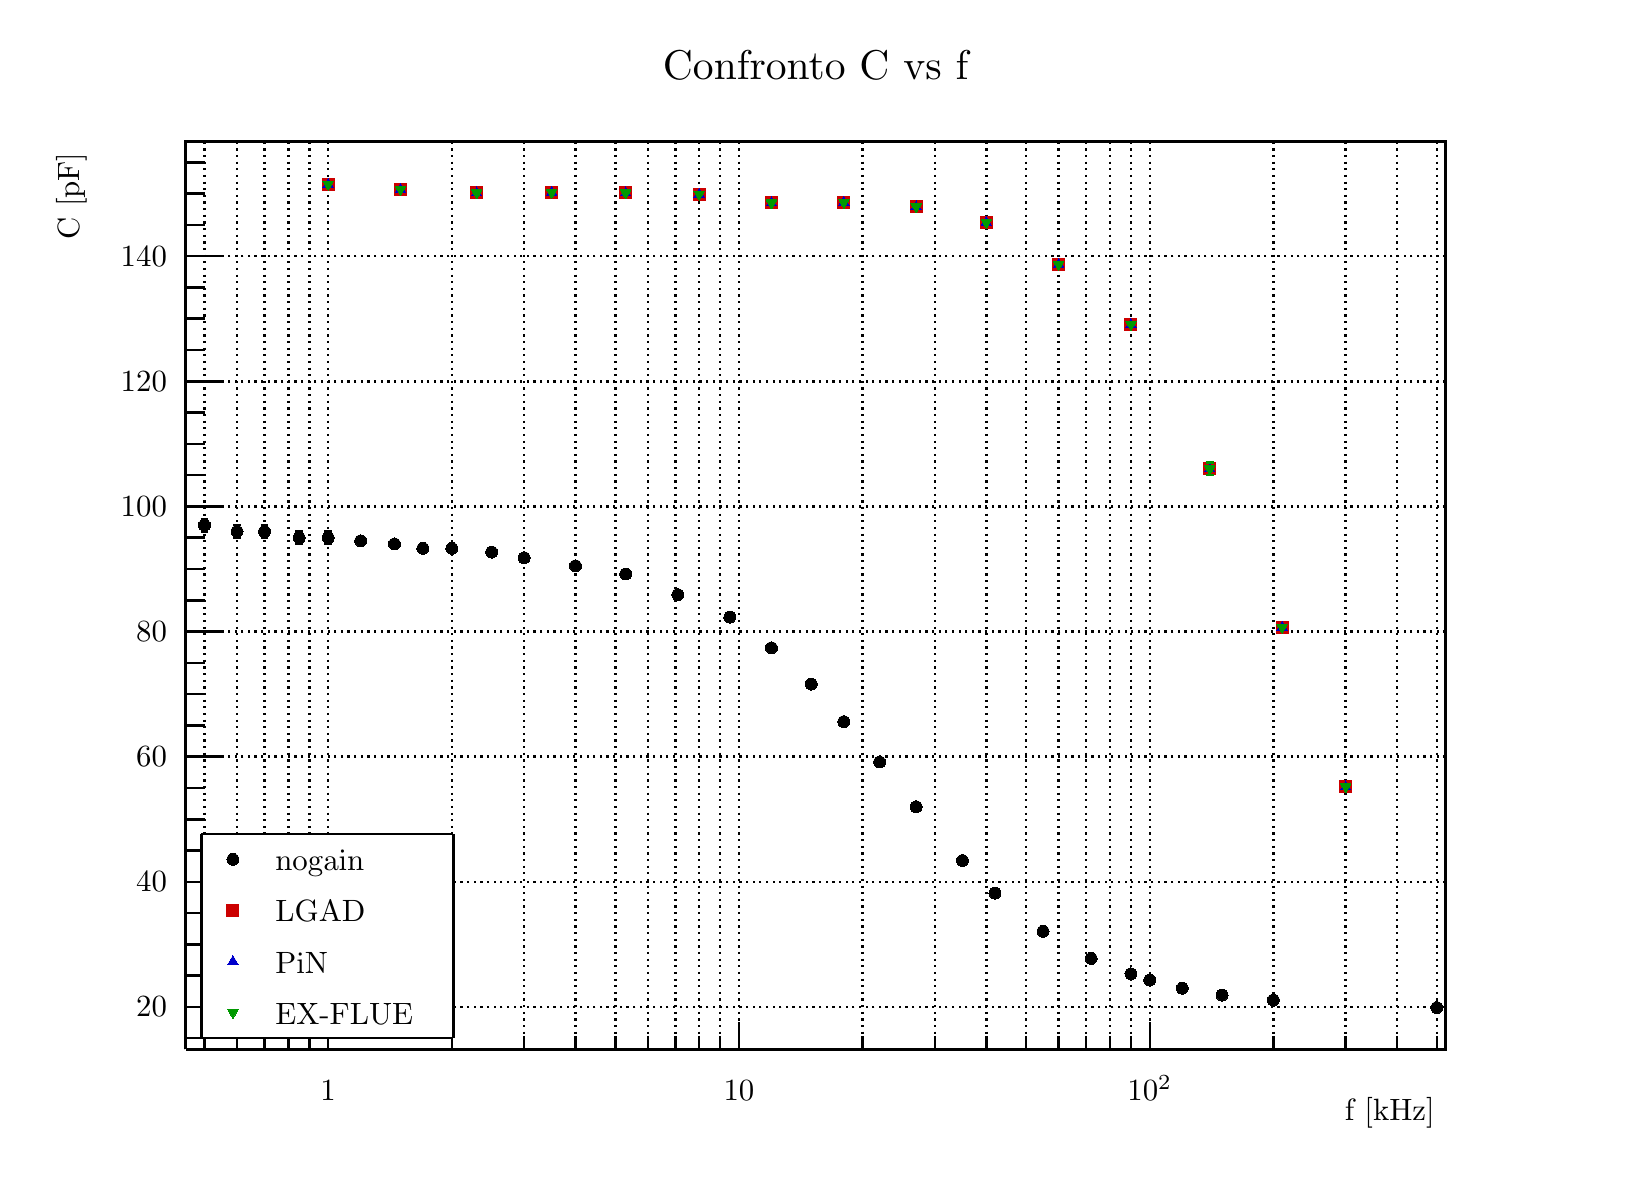
\begin{tikzpicture}
\def\CheckTikzLibraryLoaded#1{ \ifcsname tikz@library@#1@loaded\endcsname \else \PackageWarning{tikz}{usetikzlibrary{#1} is missing in the preamble.} \fi }
\CheckTikzLibraryLoaded{patterns}
\CheckTikzLibraryLoaded{plotmarks}
\pgfdeclareplotmark{cross} {
\pgfpathmoveto{\pgfpoint{-0.3\pgfplotmarksize}{\pgfplotmarksize}}
\pgfpathlineto{\pgfpoint{+0.3\pgfplotmarksize}{\pgfplotmarksize}}
\pgfpathlineto{\pgfpoint{+0.3\pgfplotmarksize}{0.3\pgfplotmarksize}}
\pgfpathlineto{\pgfpoint{+1\pgfplotmarksize}{0.3\pgfplotmarksize}}
\pgfpathlineto{\pgfpoint{+1\pgfplotmarksize}{-0.3\pgfplotmarksize}}
\pgfpathlineto{\pgfpoint{+0.3\pgfplotmarksize}{-0.3\pgfplotmarksize}}
\pgfpathlineto{\pgfpoint{+0.3\pgfplotmarksize}{-1.\pgfplotmarksize}}
\pgfpathlineto{\pgfpoint{-0.3\pgfplotmarksize}{-1.\pgfplotmarksize}}
\pgfpathlineto{\pgfpoint{-0.3\pgfplotmarksize}{-0.3\pgfplotmarksize}}
\pgfpathlineto{\pgfpoint{-1.\pgfplotmarksize}{-0.3\pgfplotmarksize}}
\pgfpathlineto{\pgfpoint{-1.\pgfplotmarksize}{0.3\pgfplotmarksize}}
\pgfpathlineto{\pgfpoint{-0.3\pgfplotmarksize}{0.3\pgfplotmarksize}}
\pgfpathclose
\pgfusepathqstroke
}
\pgfdeclareplotmark{cross*} {
\pgfpathmoveto{\pgfpoint{-0.3\pgfplotmarksize}{\pgfplotmarksize}}
\pgfpathlineto{\pgfpoint{+0.3\pgfplotmarksize}{\pgfplotmarksize}}
\pgfpathlineto{\pgfpoint{+0.3\pgfplotmarksize}{0.3\pgfplotmarksize}}
\pgfpathlineto{\pgfpoint{+1\pgfplotmarksize}{0.3\pgfplotmarksize}}
\pgfpathlineto{\pgfpoint{+1\pgfplotmarksize}{-0.3\pgfplotmarksize}}
\pgfpathlineto{\pgfpoint{+0.3\pgfplotmarksize}{-0.3\pgfplotmarksize}}
\pgfpathlineto{\pgfpoint{+0.3\pgfplotmarksize}{-1.\pgfplotmarksize}}
\pgfpathlineto{\pgfpoint{-0.3\pgfplotmarksize}{-1.\pgfplotmarksize}}
\pgfpathlineto{\pgfpoint{-0.3\pgfplotmarksize}{-0.3\pgfplotmarksize}}
\pgfpathlineto{\pgfpoint{-1.\pgfplotmarksize}{-0.3\pgfplotmarksize}}
\pgfpathlineto{\pgfpoint{-1.\pgfplotmarksize}{0.3\pgfplotmarksize}}
\pgfpathlineto{\pgfpoint{-0.3\pgfplotmarksize}{0.3\pgfplotmarksize}}
\pgfpathclose
\pgfusepathqfillstroke
}
\pgfdeclareplotmark{newstar} {
\pgfpathmoveto{\pgfqpoint{0pt}{\pgfplotmarksize}}
\pgfpathlineto{\pgfqpointpolar{44}{0.5\pgfplotmarksize}}
\pgfpathlineto{\pgfqpointpolar{18}{\pgfplotmarksize}}
\pgfpathlineto{\pgfqpointpolar{-20}{0.5\pgfplotmarksize}}
\pgfpathlineto{\pgfqpointpolar{-54}{\pgfplotmarksize}}
\pgfpathlineto{\pgfqpointpolar{-90}{0.5\pgfplotmarksize}}
\pgfpathlineto{\pgfqpointpolar{234}{\pgfplotmarksize}}
\pgfpathlineto{\pgfqpointpolar{198}{0.5\pgfplotmarksize}}
\pgfpathlineto{\pgfqpointpolar{162}{\pgfplotmarksize}}
\pgfpathlineto{\pgfqpointpolar{134}{0.5\pgfplotmarksize}}
\pgfpathclose
\pgfusepathqstroke
}
\pgfdeclareplotmark{newstar*} {
\pgfpathmoveto{\pgfqpoint{0pt}{\pgfplotmarksize}}
\pgfpathlineto{\pgfqpointpolar{44}{0.5\pgfplotmarksize}}
\pgfpathlineto{\pgfqpointpolar{18}{\pgfplotmarksize}}
\pgfpathlineto{\pgfqpointpolar{-20}{0.5\pgfplotmarksize}}
\pgfpathlineto{\pgfqpointpolar{-54}{\pgfplotmarksize}}
\pgfpathlineto{\pgfqpointpolar{-90}{0.5\pgfplotmarksize}}
\pgfpathlineto{\pgfqpointpolar{234}{\pgfplotmarksize}}
\pgfpathlineto{\pgfqpointpolar{198}{0.5\pgfplotmarksize}}
\pgfpathlineto{\pgfqpointpolar{162}{\pgfplotmarksize}}
\pgfpathlineto{\pgfqpointpolar{134}{0.5\pgfplotmarksize}}
\pgfpathclose
\pgfusepathqfillstroke
}
\definecolor{c}{rgb}{1,1,1};
\draw [color=c, fill=c] (0,0) rectangle (20,14.411);
\draw [color=c, fill=c] (2,1.4411) rectangle (18,12.9699);
\definecolor{c}{rgb}{0,0,0};
\draw [c,line width=0.9] (2,1.4411) -- (2,12.9699) -- (18,12.9699) -- (18,1.4411) -- (2,1.4411);
\definecolor{c}{rgb}{1,1,1};
\draw [color=c, fill=c] (2,1.4411) rectangle (18,12.9699);
\definecolor{c}{rgb}{0,0,0};
\draw [c,line width=0.9] (2,1.4411) -- (2,12.9699) -- (18,12.9699) -- (18,1.4411) -- (2,1.4411);
\draw [c,line width=0.9] (2,1.4411) -- (18,1.4411);
\draw [c,dash pattern=on 0.80pt off 1.60pt ,line width=0.9] (2.23872,12.9699) -- (2.23872,1.4411);
\draw [c,dash pattern=on 0.80pt off 1.60pt ,line width=0.9] (2.6518,12.9699) -- (2.6518,1.4411);
\draw [c,dash pattern=on 0.80pt off 1.60pt ,line width=0.9] (3.00106,12.9699) -- (3.00106,1.4411);
\draw [c,dash pattern=on 0.80pt off 1.60pt ,line width=0.9] (3.3036,12.9699) -- (3.3036,1.4411);
\draw [c,dash pattern=on 0.80pt off 1.60pt ,line width=0.9] (3.57046,12.9699) -- (3.57046,1.4411);
\draw [c,dash pattern=on 0.80pt off 1.60pt ,line width=0.9] (3.80918,12.9699) -- (3.80918,1.4411);
\draw [c,dash pattern=on 0.80pt off 1.60pt ,line width=0.9] (5.37964,12.9699) -- (5.37964,1.4411);
\draw [c,dash pattern=on 0.80pt off 1.60pt ,line width=0.9] (6.29829,12.9699) -- (6.29829,1.4411);
\draw [c,dash pattern=on 0.80pt off 1.60pt ,line width=0.9] (6.95009,12.9699) -- (6.95009,1.4411);
\draw [c,dash pattern=on 0.80pt off 1.60pt ,line width=0.9] (7.45567,12.9699) -- (7.45567,1.4411);
\draw [c,dash pattern=on 0.80pt off 1.60pt ,line width=0.9] (7.86875,12.9699) -- (7.86875,1.4411);
\draw [c,dash pattern=on 0.80pt off 1.60pt ,line width=0.9] (8.21801,12.9699) -- (8.21801,1.4411);
\draw [c,dash pattern=on 0.80pt off 1.60pt ,line width=0.9] (8.52055,12.9699) -- (8.52055,1.4411);
\draw [c,dash pattern=on 0.80pt off 1.60pt ,line width=0.9] (8.78741,12.9699) -- (8.78741,1.4411);
\draw [c,dash pattern=on 0.80pt off 1.60pt ,line width=0.9] (9.02613,12.9699) -- (9.02613,1.4411);
\draw [c,dash pattern=on 0.80pt off 1.60pt ,line width=0.9] (10.5966,12.9699) -- (10.5966,1.4411);
\draw [c,dash pattern=on 0.80pt off 1.60pt ,line width=0.9] (11.5152,12.9699) -- (11.5152,1.4411);
\draw [c,dash pattern=on 0.80pt off 1.60pt ,line width=0.9] (12.167,12.9699) -- (12.167,1.4411);
\draw [c,dash pattern=on 0.80pt off 1.60pt ,line width=0.9] (12.6726,12.9699) -- (12.6726,1.4411);
\draw [c,dash pattern=on 0.80pt off 1.60pt ,line width=0.9] (13.0857,12.9699) -- (13.0857,1.4411);
\draw [c,dash pattern=on 0.80pt off 1.60pt ,line width=0.9] (13.435,12.9699) -- (13.435,1.4411);
\draw [c,dash pattern=on 0.80pt off 1.60pt ,line width=0.9] (13.7375,12.9699) -- (13.7375,1.4411);
\draw [c,dash pattern=on 0.80pt off 1.60pt ,line width=0.9] (14.0044,12.9699) -- (14.0044,1.4411);
\draw [c,dash pattern=on 0.80pt off 1.60pt ,line width=0.9] (14.2431,12.9699) -- (14.2431,1.4411);
\draw [c,dash pattern=on 0.80pt off 1.60pt ,line width=0.9] (15.8135,12.9699) -- (15.8135,1.4411);
\draw [c,dash pattern=on 0.80pt off 1.60pt ,line width=0.9] (16.7322,12.9699) -- (16.7322,1.4411);
\draw [c,dash pattern=on 0.80pt off 1.60pt ,line width=0.9] (17.384,12.9699) -- (17.384,1.4411);
\draw [c,dash pattern=on 0.80pt off 1.60pt ,line width=0.9] (17.8896,12.9699) -- (17.8896,1.4411);
\draw [c,line width=0.9] (2,1.4411) -- (2,12.9699);
\draw [c,dash pattern=on 0.80pt off 1.60pt ,line width=0.9] (18,1.98103) -- (2,1.98103);
\draw [c,dash pattern=on 0.80pt off 1.60pt ,line width=0.9] (18,3.57023) -- (2,3.57023);
\draw [c,dash pattern=on 0.80pt off 1.60pt ,line width=0.9] (18,5.15942) -- (2,5.15942);
\draw [c,dash pattern=on 0.80pt off 1.60pt ,line width=0.9] (18,6.74862) -- (2,6.74862);
\draw [c,dash pattern=on 0.80pt off 1.60pt ,line width=0.9] (18,8.33782) -- (2,8.33782);
\draw [c,dash pattern=on 0.80pt off 1.60pt ,line width=0.9] (18,9.92701) -- (2,9.92701);
\draw [c,dash pattern=on 0.80pt off 1.60pt ,line width=0.9] (18,11.5162) -- (2,11.5162);
\draw [c,dash pattern=on 0.80pt off 1.60pt ,line width=0.9] (18,1.98103) -- (2,1.98103);
\draw [c,dash pattern=on 0.80pt off 1.60pt ,line width=0.9] (18,11.5162) -- (2,11.5162);
\draw [c,line width=0.9] (2,1.4411) -- (18,1.4411);
\draw [c,line width=0.9] (2.23872,1.61404) -- (2.23872,1.4411);
\draw [c,line width=0.9] (2.6518,1.61404) -- (2.6518,1.4411);
\draw [c,line width=0.9] (3.00106,1.61404) -- (3.00106,1.4411);
\draw [c,line width=0.9] (3.3036,1.61404) -- (3.3036,1.4411);
\draw [c,line width=0.9] (3.57046,1.61404) -- (3.57046,1.4411);
\draw [c,line width=0.9] (3.80918,1.78697) -- (3.80918,1.4411);
\draw [anchor=base] (3.80918,0.789004) node[scale=1.11327, color=c, rotate=0]{1};
\draw [c,line width=0.9] (5.37964,1.61404) -- (5.37964,1.4411);
\draw [c,line width=0.9] (6.29829,1.61404) -- (6.29829,1.4411);
\draw [c,line width=0.9] (6.95009,1.61404) -- (6.95009,1.4411);
\draw [c,line width=0.9] (7.45567,1.61404) -- (7.45567,1.4411);
\draw [c,line width=0.9] (7.86875,1.61404) -- (7.86875,1.4411);
\draw [c,line width=0.9] (8.21801,1.61404) -- (8.21801,1.4411);
\draw [c,line width=0.9] (8.52055,1.61404) -- (8.52055,1.4411);
\draw [c,line width=0.9] (8.78741,1.61404) -- (8.78741,1.4411);
\draw [c,line width=0.9] (9.02613,1.78697) -- (9.02613,1.4411);
\draw [anchor=base] (9.02613,0.789004) node[scale=1.11327, color=c, rotate=0]{10};
\draw [c,line width=0.9] (10.5966,1.61404) -- (10.5966,1.4411);
\draw [c,line width=0.9] (11.5152,1.61404) -- (11.5152,1.4411);
\draw [c,line width=0.9] (12.167,1.61404) -- (12.167,1.4411);
\draw [c,line width=0.9] (12.6726,1.61404) -- (12.6726,1.4411);
\draw [c,line width=0.9] (13.0857,1.61404) -- (13.0857,1.4411);
\draw [c,line width=0.9] (13.435,1.61404) -- (13.435,1.4411);
\draw [c,line width=0.9] (13.7375,1.61404) -- (13.7375,1.4411);
\draw [c,line width=0.9] (14.0044,1.61404) -- (14.0044,1.4411);
\draw [c,line width=0.9] (14.2431,1.78697) -- (14.2431,1.4411);
\draw [anchor=base] (14.2431,0.789004) node[scale=1.11327, color=c, rotate=0]{$10^{2}$};
\draw [c,line width=0.9] (15.8135,1.61404) -- (15.8135,1.4411);
\draw [c,line width=0.9] (16.7322,1.61404) -- (16.7322,1.4411);
\draw [c,line width=0.9] (17.384,1.61404) -- (17.384,1.4411);
\draw [c,line width=0.9] (17.8896,1.61404) -- (17.8896,1.4411);
\draw [anchor= east] (18,0.634085) node[scale=1.11327, color=c, rotate=0]{f [kHz]};
\draw [c,line width=0.9] (2,1.4411) -- (2,12.9699);
\draw [c,line width=0.9] (2.48,1.98103) -- (2,1.98103);
\draw [c,line width=0.9] (2.24,2.37833) -- (2,2.37833);
\draw [c,line width=0.9] (2.24,2.77563) -- (2,2.77563);
\draw [c,line width=0.9] (2.24,3.17293) -- (2,3.17293);
\draw [c,line width=0.9] (2.48,3.57023) -- (2,3.57023);
\draw [c,line width=0.9] (2.24,3.96753) -- (2,3.96753);
\draw [c,line width=0.9] (2.24,4.36483) -- (2,4.36483);
\draw [c,line width=0.9] (2.24,4.76213) -- (2,4.76213);
\draw [c,line width=0.9] (2.48,5.15942) -- (2,5.15942);
\draw [c,line width=0.9] (2.24,5.55672) -- (2,5.55672);
\draw [c,line width=0.9] (2.24,5.95402) -- (2,5.95402);
\draw [c,line width=0.9] (2.24,6.35132) -- (2,6.35132);
\draw [c,line width=0.9] (2.48,6.74862) -- (2,6.74862);
\draw [c,line width=0.9] (2.24,7.14592) -- (2,7.14592);
\draw [c,line width=0.9] (2.24,7.54322) -- (2,7.54322);
\draw [c,line width=0.9] (2.24,7.94052) -- (2,7.94052);
\draw [c,line width=0.9] (2.48,8.33782) -- (2,8.33782);
\draw [c,line width=0.9] (2.24,8.73512) -- (2,8.73512);
\draw [c,line width=0.9] (2.24,9.13241) -- (2,9.13241);
\draw [c,line width=0.9] (2.24,9.52971) -- (2,9.52971);
\draw [c,line width=0.9] (2.48,9.92701) -- (2,9.92701);
\draw [c,line width=0.9] (2.24,10.3243) -- (2,10.3243);
\draw [c,line width=0.9] (2.24,10.7216) -- (2,10.7216);
\draw [c,line width=0.9] (2.24,11.1189) -- (2,11.1189);
\draw [c,line width=0.9] (2.48,11.5162) -- (2,11.5162);
\draw [c,line width=0.9] (2.48,1.98103) -- (2,1.98103);
\draw [c,line width=0.9] (2.24,1.58373) -- (2,1.58373);
\draw [c,line width=0.9] (2.48,11.5162) -- (2,11.5162);
\draw [c,line width=0.9] (2.24,11.9135) -- (2,11.9135);
\draw [c,line width=0.9] (2.24,12.3108) -- (2,12.3108);
\draw [c,line width=0.9] (2.24,12.7081) -- (2,12.7081);
\draw [anchor= east] (1.9,1.98103) node[scale=1.11327, color=c, rotate=0]{20};
\draw [anchor= east] (1.9,3.57023) node[scale=1.11327, color=c, rotate=0]{40};
\draw [anchor= east] (1.9,5.15942) node[scale=1.11327, color=c, rotate=0]{60};
\draw [anchor= east] (1.9,6.74862) node[scale=1.11327, color=c, rotate=0]{80};
\draw [anchor= east] (1.9,8.33782) node[scale=1.11327, color=c, rotate=0]{100};
\draw [anchor= east] (1.9,9.92701) node[scale=1.11327, color=c, rotate=0]{120};
\draw [anchor= east] (1.9,11.5162) node[scale=1.11327, color=c, rotate=0]{140};
\draw [anchor= east] (0.54812,12.9699) node[scale=1.11327, color=c, rotate=90]{C [pF]};
\draw [c,line width=0.9] (2.23871,8.17462) -- (2.23871,8.1789);
\draw [c,line width=0.9] (2.23871,8.02425) -- (2.23871,8.01998);
\draw [c,line width=0.9] (2.18859,8.1789) -- (2.28884,8.1789);
\draw [c,line width=0.9] (2.18859,8.01998) -- (2.28884,8.01998);
\draw [c,line width=0.9] (2.6518,8.09517) -- (2.6518,8.09944);
\draw [c,line width=0.9] (2.6518,7.94479) -- (2.6518,7.94052);
\draw [c,line width=0.9] (2.60167,8.09944) -- (2.70192,8.09944);
\draw [c,line width=0.9] (2.60167,7.94052) -- (2.70192,7.94052);
\draw [c,line width=0.9] (3.00106,8.09517) -- (3.00106,8.09944);
\draw [c,line width=0.9] (3.00106,7.94479) -- (3.00106,7.94052);
\draw [c,line width=0.9] (2.95093,8.09944) -- (3.05118,8.09944);
\draw [c,line width=0.9] (2.95093,7.94052) -- (3.05118,7.94052);
\draw [c,line width=0.9] (3.44096,8.01571) -- (3.44096,8.01998);
\draw [c,line width=0.9] (3.44096,7.86533) -- (3.44096,7.86106);
\draw [c,line width=0.9] (3.39083,8.01998) -- (3.49108,8.01998);
\draw [c,line width=0.9] (3.39083,7.86106) -- (3.49108,7.86106);
\draw [c,line width=0.9] (3.80917,8.01571) -- (3.80917,8.01998);
\draw [c,line width=0.9] (3.80917,7.86533) -- (3.80917,7.86106);
\draw [c,line width=0.9] (3.75905,8.01998) -- (3.8593,8.01998);
\draw [c,line width=0.9] (3.75905,7.86106) -- (3.8593,7.86106);
\foreach \P in {(2.23871,8.09944), (2.6518,8.01998), (3.00106,8.01998), (3.44096,7.94052), (3.80917,7.94052), (4.22226,7.90079), (4.65102,7.86106), (5.01141,7.80544), (5.37963,7.80544), (5.88521,7.75776), (6.29829,7.68625), (6.95009,7.58295),
 (7.58768,7.47965), (8.25014,7.21743), (8.90991,6.93138), (9.43921,6.54202), (9.94478,6.08116), (10.3579,5.6044), (10.8125,5.09188), (11.2765,4.52375), (11.8645,3.84039), (12.2776,3.42561), (12.8886,2.94091), (13.4988,2.59764), (14.0044,2.40217),
 (14.2431,2.32271), (14.6562,2.21941), (15.1617,2.13201), (15.8135,2.06844), (17.8896,1.97309)}{\draw[mark options={color=c,fill=c},mark size=2.162162pt, line width=0.000000pt, mark=*] plot coordinates {\P};}
\definecolor{c}{rgb}{0.8,0,0};
\draw [c,line width=0.9] (15.0054,8.88976) -- (15.0054,8.89403);
\draw [c,line width=0.9] (15.0054,8.73939) -- (15.0054,8.73512);
\draw [c,line width=0.9] (14.9553,8.89403) -- (15.0555,8.89403);
\draw [c,line width=0.9] (14.9553,8.73512) -- (15.0555,8.73512);
\foreach \P in {(3.80917,12.43), (4.72783,12.3664), (5.69629,12.3188), (6.64755,12.3267), (7.58768,12.3188), (8.52055,12.3052), (9.43921,12.1916), (10.3579,12.1996), (11.2765,12.1439), (12.167,11.9453), (13.0857,11.4129), (14.0044,10.6501),
 (15.0054,8.81458), (15.9241,6.80424), (16.7322,4.77802)}{\draw[mark options={color=c,fill=c},mark size=2.162162pt, line width=0.000000pt, mark=square*] plot coordinates {\P};}
\definecolor{c}{rgb}{0,0,0.8};
\draw [c,line width=0.9] (15.0054,8.88976) -- (15.0054,8.89403);
\draw [c,line width=0.9] (15.0054,8.73939) -- (15.0054,8.73512);
\draw [c,line width=0.9] (14.9553,8.89403) -- (15.0555,8.89403);
\draw [c,line width=0.9] (14.9553,8.73512) -- (15.0555,8.73512);
\foreach \P in {(3.80917,12.43), (4.72783,12.3664), (5.69629,12.3188), (6.64755,12.3267), (7.58768,12.3188), (8.52055,12.3052), (9.43921,12.1916), (10.3579,12.1996), (11.2765,12.1439), (12.167,11.9453), (13.0857,11.4129), (14.0044,10.6501),
 (15.0054,8.81458), (15.9241,6.80424), (16.7322,4.77802)}{\draw[mark options={color=c,fill=c},mark size=2.162162pt, line width=0.000000pt, mark=triangle*] plot coordinates {\P};}
\definecolor{c}{rgb}{0,0.6,0};
\draw [c,line width=0.9] (15.0054,8.88976) -- (15.0054,8.89403);
\draw [c,line width=0.9] (15.0054,8.73939) -- (15.0054,8.73512);
\draw [c,line width=0.9] (14.9553,8.89403) -- (15.0555,8.89403);
\draw [c,line width=0.9] (14.9553,8.73512) -- (15.0555,8.73512);
\foreach \P in {(3.80917,12.43), (4.72783,12.3664), (5.69629,12.3188), (6.64755,12.3267), (7.58768,12.3188), (8.52055,12.3052), (9.43921,12.1916), (10.3579,12.1996), (11.2765,12.1439), (12.167,11.9453), (13.0857,11.4129), (14.0044,10.6501),
 (15.0054,8.81458), (15.9241,6.80424), (16.7322,4.77802)}{\draw[mark options={color=c,fill=c,rotate=180},mark size=2.162162pt, line width=0.000000pt, mark=triangle*] plot coordinates {\P};}
\definecolor{c}{rgb}{1,1,1};
\draw [color=c, fill=c] (2.2,1.58521) rectangle (5.4,4.1792);
\definecolor{c}{rgb}{0,0,0};
\draw [c,line width=0.9] (2.2,1.58521) -- (5.4,1.58521);
\draw [c,line width=0.9] (5.4,1.58521) -- (5.4,4.1792);
\draw [c,line width=0.9] (5.4,4.1792) -- (2.2,4.1792);
\draw [c,line width=0.9] (2.2,4.1792) -- (2.2,1.58521);
\draw [anchor=base west] (3,3.70904) node[scale=1.11327, color=c, rotate=0]{nogain};
\foreach \P in {(2.6,3.85495)}{\draw[mark options={color=c,fill=c},mark size=2.162162pt, line width=0.000000pt, mark=*] plot coordinates {\P};}
\draw [anchor=base west] (3,3.06054) node[scale=1.11327, color=c, rotate=0]{LGAD};
\definecolor{c}{rgb}{0.8,0,0};
\foreach \P in {(2.6,3.20645)}{\draw[mark options={color=c,fill=c},mark size=2.162162pt, line width=0.000000pt, mark=square*] plot coordinates {\P};}
\definecolor{c}{rgb}{0,0,0};
\draw [anchor=base west] (3,2.41205) node[scale=1.11327, color=c, rotate=0]{PiN};
\definecolor{c}{rgb}{0,0,0.8};
\foreach \P in {(2.6,2.55796)}{\draw[mark options={color=c,fill=c},mark size=2.162162pt, line width=0.000000pt, mark=triangle*] plot coordinates {\P};}
\definecolor{c}{rgb}{0,0,0};
\draw [anchor=base west] (3,1.76355) node[scale=1.11327, color=c, rotate=0]{EX-FLUE};
\definecolor{c}{rgb}{0,0.6,0};
\foreach \P in {(2.6,1.90946)}{\draw[mark options={color=c,fill=c,rotate=180},mark size=2.162162pt, line width=0.000000pt, mark=triangle*] plot coordinates {\P};}
\definecolor{c}{rgb}{0,0,0};
\draw (10,13.9427) node[scale=1.50291, color=c, rotate=0]{Confronto C vs f};
\end{tikzpicture}
%\end{document}
